\chapterquote{%
The two operations of our understanding, intuition and deduction, on which alone we have said we must rely in the acquisition of knowledge.}
{-- Rene Descartes, \textit{Key Philosophical Writings} (1997)}

The purpose of this chapter is to characterize the distribution of the interference in a typical packet transmitted through an asynchronous channel, where fixed-length packets arrive according to a Poisson process.
%
Although simple and theoretical, because we do not consider spatial positions or fading effects, we deemed it important to build intuition on the structure of our main problem of characterizing the spatio-temporal interference on Poisson networks.

\newpage

\section{The Interference Model}

Let $\tau$ be the transmission time of the packets that use the channel. Let the homogeneous Poisson point process $\Pi$ on $\R$ with density $\lambda > 0$ be the times for which a transmission starts.

We are interested in the stochastic process $\{I_0(t)\}_{t\in[0,\tau]}$, which corresponds to the number of simultaneous interfering packets on a typical packet that started its transmission at $t=0$. Then, the interference is defined as a shot-noise field given by
\begin{align} \label{eq:interf_I0}
    I_0(t) \triangleq \sum_{x\in\Pi^!_0} \ind_{[0,\tau)}(t-x), \quad t\in[0,\tau),
\end{align}
where $\Pi^!_0$ is the \textit{reduced Palm version} of $\Pi$, i.e., $\Pi$ conditioned to having a point at the origin and excluding it.
%
Slivnyak's theorem (Theorem~\ref{th:slivnyak}) guarantees that the distribution of $\Pi^!_0(\cdot)$ is the same as $\Pi(\cdot)$ for a Poisson point process.

In view of the general network model of Chapter~\ref{cap:P2_00}, we provide two of many possible scenarios for which this model can be applied.

\begin{example}
    Consider a stationary bipolar high-mobility Poisson network with density of transmitters $\lambda_{\S}>0$ on the plane $\S=\R^2$, and transmission time $\tau_i = \tau$ and transmission power $P_i \equiv 1$ for every user $i\in\N$.
    
    Suppose packets arrive at each transmitter according to a Poisson point process of density $a>0$ on time $\T = \R$ and there is no buffer in the transmitters, thus packets are transmitted upon arrival and discarded afterward (independently of successful transmission), i.e., $A_{i} = T_{i} = T^*_{i}$ for all users $i\in\N$.
    
    In a scenario without small-scale fading ($H_{ij} \equiv 1$ for all $i,j\in\N$) and with path loss function $\ell(r) = \ind\{r < r_0\}$, $r_0>0$,
    %
    the interference model presented in \eqref{eq:interf_I0} applies to this network with $\lambda = \pi r_0^2\,\lambda_\S\,a$.
\end{example}

\begin{example}
    Consider a stationary bipolar static network with $n\in\N$ transmitters and $n$ receivers on a small disk of radius $1$ ($\S=\{x\in\R^2: ||x|| < 1\}$) such that small-scale fading and path loss can be ignored, i.e., $H_{ij} \equiv 1$ for all $i,j\in\{1,2,\dots,n\}$ and $\ell \equiv 1$.
    %
    Further, the transmission time $\tau_i = \tau$ and transmission power $P_i \equiv 1$ for every user $i\in\{1,2,\dots,n\}$.
    
    Suppose that the medium access protocol is to transmit a packet after an iid exponentially distributed time of parameter $\lambda_p > 0$ after the last transmission, i.e., $T_i$ is a Poisson point process of density $\lambda_p$ on $\T = \R$ for each $i\in\{1,2,\dots,n\}$.

    Let us consider that each transmitter has a buffer and we have saturated traffic, i.e., all transmitter's queues are non-empty at all times, so $A_i$ does not matter and $T_i^* = T_i$, because there is always a packet to transmit.
    %
    Then, the interference model presented in \eqref{eq:interf_I0} applies to this network with $\lambda = n\lambda_p$.
\end{example}

The above examples do not specify the transmission probability model $\mathscr{S}$. This is not done because it depends on the adopted model for success probability and each of the following sections presents a different model.

Although we provided only two scenarios, it is not hard to see that we must have a stationary network with a single user class, which implies that the throughput is given by the product of the traffic with the transmission success probability, i.e., $\mathscr{T} = \upsilon\,p_s$.

Let us begin the characterization of $I_0$ through its auto-covariance function, which is given by, for $\Delta t\in(-\tau,\tau)$,
\begin{align*}
    \mathrm{K}_{I_0}(\Delta t)
        &\triangleq \E[I_0(t) I_0(t+\Delta t)] - \E[I_0(t)] \E[I_0(t+\Delta t)], \quad t\in[0,\tau)\cap[-\Delta t, \tau-\Delta t),\\
        &= \sum_{k_0\ge 0}\sum_{k_1\ge 0}\sum_{k_2\ge 0} (k_0+k_1)(k_0+k_2) \frac{\lambda^{k_0}(\tau-|\Delta t|)^{k_0}}{k_0!}\,\euler^{-\lambda(\tau-|\Delta t|)}\\
        &\hspace{30mm} \times\frac{\lambda^{k_1}|\Delta t|^{k_1}}{k_1!}\euler^{-\lambda|\Delta t|} \,\frac{\lambda^{k_2}|\Delta t|^{k_2}}{k_2!}\euler^{-\lambda|\Delta t|} - (\lambda\tau)^2\\
        &= \lambda(\tau - |\Delta t|),
\end{align*}
where we have used the identity $\displaystyle\sum_{k\ge0} \frac{x^k}{k!} = \euler^x$, for any $x\in\R^*$.

As expected of a Poisson point process, which is independent across space (or, in this case, time), the factor responsible for correlation in the stochastic process $I_0$ is related to the duration $\tau$ of each transmitted packet. That is why $\mathrm{K}_{I_0}(\tau) = 0$.

\begin{remark} \label{remark:Ch5_I0}
    To illustrate a (rarely mentioned) dichotomy, we have calculated \textit{(i)} the Laplace transform of $I_0$ on the interval $[0,\tau)$ and \textit{(ii)} the Laplace transform of the distribution of $I_0(t)$ at $t\in[0,\tau)$.
    %
    On the one hand, \textit{(i)} characterizes the stochastic process on time, but not in distribution.
    %
    On the other hand, \textit{(ii)} characterizes the distribution of the stochastic process at a point in time, but we cannot analyze the process as a whole, which is essential to decide whether a transmission is successful.
    %
    The calculations follow.
    
    \textit{(i)} Let $s\in\C\backslash\{0\}$. The Laplace transform of $I_0$ on the interval $[0,\tau)$ is given by
    \begin{align}
        \mathscr{L}\{I_0\}(s)
            &= \int_0^\tau I_0(t)\,\euler^{-s t}\,\d t \nonumber\\
            &= \sum_{x\in\Pi} \int_0^\tau \ind_{[0,\tau]}(t-x)\,\euler^{-s t}\,\d t\nonumber\\
            &= \sum_{x\in\Pi} \left(\euler^{-s \lfloor -x\rceil_0^\tau} - \euler^{-s \lfloor \tau-x \rceil_0^\tau} \right)\frac{\euler^{-s x}}{s}, \label{eq:Ch5_LT_I0}
    \end{align}
    where $\lfloor \cdot\rceil_a^b = \max\{\min\{\cdot,b\},a\}$.
    
    \textit{(ii)} Let $s\in\C$. The Laplace transform of the distribution of $I_0(t)$, $t\in[0,\tau)$ is
    \begin{align*}
        \mathscr{L}_{I_0(t)}(s) &= \E[\euler^{-s\,I_0(t)}]\\
            &= \E\!\left[-\sum_{x\in\Pi} s\ind_{[0,\tau)}(t-x) \right]\\
            &= \exp\!\left(-\int_\R \left(1 - \euler^{-s\ind_{[0,\tau)}(t-x)}\right)\lambda\,\d x \right)\\
            &= \exp\!\left(-\int_0^\tau \left(1 - \euler^{-s}\right)\lambda\,\d x \right)\\
            &= \euler^{-\lambda\tau(1-\euler^{-s})},
    \end{align*}
    % Then, using Campbell Theorem (Theorem~\ref{th:campbell}),
    % \begin{align*}
    %     \E\!\left[\frac{1}{\tau}\mathscr{L}\{I_0(t)\}(s)\right]
    %         &= \int_\R \left(\euler^{-s \lfloor -x\rceil_0^\tau} - \euler^{-s \lfloor \tau-x \rceil_0^\tau} \right)\frac{\euler^{-s x}}{\tau s} \lambda\,\d x \\
    %         &= \lambda\tau \frac{1-\euler^{-\tau s}}{\tau s}.
    % \end{align*}
    where we have used Campbell's theorem (Theorem~\ref{th:campbell}) in the third equality.
    
    To analyze a successful transmission we need the characterization of the interference both in distribution and in time. As shown, it is easy to do one of them, however, both at the same time (e.g. calculating the Laplace transform of the distribution of \eqref{eq:Ch5_LT_I0}) does not yield a tractable formula.
\end{remark}

As illustrated in Remark~\ref{remark:Ch5_I0}, it is hard to characterize the distribution of $I_0$ on the interval $[0,\tau)$ and in distribution concomitantly.
%
Thus, we shall define a meaningful functional (related to a success probability) that receives as argument $I_0$ and give us a real number, e.g. the mean value of $I_0$ on $[0,\tau)$.
%
Then, we characterize the distribution of this functional\footnote{In the general model of Chapter~\ref{cap:P2_00} the transmission success probability model $\mathscr{S}$ receives as argument the $\SIR$ instead of the interference $I_0$, however, this is easy to adapt, because the $\SIR$ includes the interference.}.

% % % % % % % % % % % % % % % % % % % % % 
\section{Error Correcting Code model}

In the Error Correcting Code model (ECC model) we assume that a packet is successfully transmitted if the proportion of the packet that was affected by interference is smaller than or equal to $\beta\in[0,1)$. %, i.e., the transmission fails if the proportion of the transmission time subjected to interference is greater than $\beta$.
%
Thus, the transmission success probability is given by $p_s = \P\!\left(\overline{S_0} \le \beta\right)$, where the random variable $\overline{S_0}$ is the proportion of the packet that was affected by interference and is defined as
\begin{align}\label{eq:ECC_I}
    \overline{S_0} \triangleq \frac{1}{\tau}\int_0^\tau \ind\{I_0(t) > 0\}\,\d t.
\end{align}
%
\begin{figure}[htb]
    \centering
    \if\printfig1
        \includegraphics{Figures/Ch5_PacketsRandomChannel.pdf}
    \else
        \includegraphics[draft]{Figures/Ch5_PacketsRandomChannel.pdf}
    \fi
    \caption{An early and late interfering packets with respect to the typical packet. The hachured regions correspond to packet overlapping. If $E+L>\beta\tau$, then the packet transmission fails.}
    \label{fig:P2_diagram_ECC}
\end{figure}%

~\\

\begin{theorem} \label{th:F_S0}
    The cumulative distribution function of $\overline{S_0}$ is
    \begin{align*}
        F_{\overline{S_0}}(x) = 
        \begin{cases}
            0, & \text{if } x < 0, \\
            (1 + \upsilon\,x)\,\euler^{-\upsilon\,(2-x)}, & \text{if } 0 \le x < 1,\\
            1, & \text{if } x \ge 1,
        \end{cases}
    \end{align*}
    where $\upsilon = \lambda\tau$.
\end{theorem}
%
\begin{proof}
    Since $\Pi$ is a Poisson point process on $\R$, the inter-arrival times follow iid exponential distributions of parameter $\lambda$. This can be shown through the void probabilities of the PPP, i.e., $\P(\Pi((0,t))=0) = \euler^{-\lambda t}$.
    
    Let the inter-arrival time of the early interferer and the late interferer be represented by the random variables $T_E\sim\mathscr{E}(\lambda)$ and $T_L\sim\mathscr{E}(\lambda)$, respectively.
    %
    Then, the superposition of the late interfering packet with the typical packet is given by $L = (\tau - T_L)_+$, where $(\cdot)_+ = \max\{\cdot,0\}$ as illustrated in Fig.~\ref{fig:P2_diagram_ECC}. Analogously for the early interferer $E = (\tau - T_E)_+$.
    %
    Thus, the cdf of $E$ and $L$ is
    \[
        F_E(t) = F_L(t) = % \ind\{t > \tau\} + \ind\{0\le t \le \tau\} \euler^{-\lambda(\tau-t)} =
        \begin{cases}
            0, &\text{if } t < 0 \\
            \euler^{-\lambda(\tau-t)}, &\text{if } 0 \le t < \tau,\\
            1, &\text{if } t \ge \tau.
        \end{cases}
    \]
    Note there is a discontinuity at $t=0$, thus the density does not exist with respect to the Lebesgue measure. Then, it is convenient to use the Lebesgue–-Stieltjes notation (Definition~\ref{def:lebesgue-stieltjes}).
    
    From \eqref{eq:ECC_I} we can see that $\overline{S_0}\,\tau = \max\{E+L,\tau\}$. Thus, for $x\in[0,1)$, we have that
    \begin{align*}
        \qquad 
        \P(\overline{S_0} \le x)
            &= \P(\max\{E+L,\tau\} \le x\,\tau) \\
            &= \P(E+L \le x\,\tau) &&\hspace{-10mm}\text{as }\tau > x\,\tau\\
            &= \int F_E(x\,\tau - t)\,\d F_L(t) &&\hspace{-10mm}\text{as $E$ and $L$ are independent}\\
            &= \euler^{-\lambda(\tau-x\,\tau)} \euler^{-\lambda\tau} + \int_0^{x\,\tau} \euler^{-\lambda(\tau-x\,\tau+t)} \lambda\euler^{-\lambda(\tau-t)}\d t \\
            &= (1+\lambda\tau\,x)\,\euler^{-\lambda\tau(2-x)}.
    \end{align*}
    The cases for which $x\notin[0,1)$ are trivial.
\end{proof}

% Note that the random variable $\overline{S_0}$ does not admit a density with respect to the Lebesgue measure, because of the discontinuities of the cdf at $0$ and $1$, that is why we used the Lebesgue--Stieltjes notation.

\begin{proposition}
	In the ECC model, where $\beta\in[0,1)$, the transmission success probability and throughput is given, respectively, by
    \begin{align*} \label{AlohaECC_thr}
        p_s     &= (1 + \beta\,\upsilon)\,\euler^{-(2-\beta)\,\upsilon},\\
    	\mathscr{T} &= \upsilon\,(1 + \beta\,\upsilon)\,\euler^{-(2-\beta)\,\upsilon},
    \end{align*}
    where $\upsilon = \lambda\tau$ is the occupation rate of the channel.
    
    Further, the unique and global maximum throughput is achieved when $\upsilon = \upsilon^*$, where
    \begin{equation*} \label{AlohaECC_max}
	    \upsilon^* = \frac{\sqrt{(2-\beta)^2+4\beta^2}-(2-3\beta)}{2\beta\,(2-\beta)}.
    \end{equation*}
\end{proposition}
\begin{proof}
    The transmission success probability and throughput follow directly from Theorem~\ref{th:F_S0} along with $p_s = \P(\overline{S_0}\le\beta) = F_{\overline{S_0}}(\beta)$ and $\mathscr{T} = \lambda\tau\,p_s$.
    
    Then, we use Theorem~\ref{th:unique_opt} to verify that the throughput has a unique local maximum which is a global maximum.
\end{proof}

If we let $\beta = 0$ in the ECC model we recover the unslotted ALOHA model \cite{abramson1970aloha}.
%
On the other hand, to achieve the maximum throughput of the slotted ALOHA, which is $1/\euler$, we must have $\beta \approx 0.56$.

Figures \ref{fig:P2_ECC} and \ref{fig:P2_ECC_ps} show the throughput $\mathscr{T}$ as a function of the traffic $\upsilon$ and as a function of the transmission success probability $p_s$, respectively.
%
As expected, the throughput grows when the system is more robust (when $\beta$ increases), even if we consider a fixed transmission success probability.

\begin{figure}[htb]
    \centering
    \if\printfig1
        % \input{Plots/Ch5_ECC.tex}
        \includegraphics[]{Figures/Ch5_ECC.pdf}
    \else
        \includegraphics[draft, width=\textwidth]{Figures/Ch5_ECC.pdf}
    \fi
    \caption{Throughput $\mathscr{T}$ of the ECC model as a function of occupation rate of the channel $\upsilon$ for different values of $\beta$.}
    \label{fig:P2_ECC}
\end{figure}%
%
\begin{figure}[htb]
    \centering
    \if\printfig1
        % \input{Plots/Ch5_ECC_ps.tex}
        \includegraphics[]{Figures/Ch5_ECC_ps.pdf}
    \else
        \includegraphics[draft, width=\textwidth]{Figures/placeholder.png}
    \fi
    \caption{Parametric curve of the throughput $\mathscr{T}$ and the transmission success probability $p_s$ as we vary $\upsilon$ in the ECC model for different values of $\beta$.}
    \label{fig:P2_ECC_ps}
\end{figure}

% % % % % % % % % % % % % % % % % % % % % 
\section{Average Interference model}
\label{sec:AI_model}

In the Average Interference model (AI model) we assume that a packet is successfully transmitted if the average of the received interference does not exceed the threshold $\beta \ge 0$.
%
Thus, the transmission success probability is given by $p_s = \P(\overline{I_0}\le\beta)$, where the random variable $\overline{I_0}$ is the mean interference on the typical packet and is defined as
\begin{align}\label{eq:AI_I}
    \overline{I_0} \triangleq \frac{1}{\tau}\int_0^\tau I_0(t)\,\d t.
\end{align}

\begin{theorem} \label{th:F_I0}
    The cumulative distribution function of $\overline{I_0}$ is given by the finite sum
    \begin{equation*}
    	F_{\overline{I_0}}(x) = \euler^{-2\upsilon} \sum_{k=0}^{\lfloor x \rfloor} \dfrac{(-1)^k}{k!} \left(\sqrt{2\,\upsilon\,(x-k)}\right)^k \cal{I}_k\!\left(\sqrt{8\,\upsilon\,(x-k)}\right),\quad x \geq 0,
    \end{equation*}
    where $\cal{I}_k$ is the $k$th order modified Bessel function of the first kind\footnote{Let $k\in\N$. The $k$th order modified Bessel function of the first kind is defined as \vspace{-2mm}\[\cal{I}_k(x) \triangleq \frac{1}{\pi}\int_0^\pi \euler^{x\cos\theta}\cos(k\theta)\,\d\theta,\quad x\in\R.\vspace{-3mm}\]}, $\lfloor \cdot \rfloor$ is the floor function\footnote{The floor function returns the biggest integer less than or equal to the argument.}, and $\upsilon = \lambda\tau$.
\end{theorem}
\begin{proof}
    From \eqref{eq:interf_I0} and \eqref{eq:AI_I}, we have that
    \begin{align*}\label{eq:AI_I}
        \overline{I_0} 
            &= \frac{1}{\tau}\int_0^\tau \sum_{x\in\Pi} \ind_{[0,\tau]}(t-x)\,\d t \\
            &= \frac{1}{\tau}\sum_{x\in\Pi} \int_0^\tau  \ind_{[0,\tau]}(t-x)\,\d t \\
            &= \frac{1}{\tau}\sum_{x\in\Pi\cap[-\tau,\tau]} (\tau - |x|),
    \end{align*}
    where we used the Fubini--Tonelli theorem (Theorem~\ref{th:fubini-tonelli}) to interchange the sum with the integral, because we have positive terms.
    %
    Note that the term $(\tau - |x|)$ gives the superposition time between an interfering packet and the typical packet.
    
    Now, using the Campbell theorem (Theorem~\ref{th:campbell}) we have that the Laplace--Stieltjes transform of the distribution of $\overline{I_0}$ is
    \begin{align*}
    	\E\!\left[\euler^{-s \overline{I_0}}\right]	&= \exp\!\left[ -\int_{-\tau}^\tau(1-\euler^{-s(1-|x|/\tau)}) \,\lambda\,dx \right] \\
        				&= \exp\!\left[ -2\upsilon\left( 1 - \frac{1-\euler^{-s}}{s} \right) \right],\quad s\in\C \backslash \{0\},
    \end{align*}
    where we used that the traffic $\upsilon = \lambda\tau$.
    
    Using the power series expansion of the exponential function on $\exp(-2\upsilon\,\euler^{-s}/s)$ and dividing by $s$ both sides of the equation, we can rewrite it as
    \begin{equation*}
    	\frac{1}{s}\E\!\left[\euler^{-s \overline{I_0}}\right] = \euler^{-2\upsilon} \sum_{k\geq0} \frac{(-2\upsilon)^k}{k!} \frac{\euler^{2\upsilon/s}}{s^{k+1}}\,\euler^{-k s},\quad s\in\C \backslash \{0\}.
    \end{equation*}
    
    % Para $k$ suficientemente grande, os valores absolutos dos termos dessa série podem ser limitados por cima pela função $e^-s$. Logo, podemos aplicar o teorema da convergência dominada para calcular a transformada de Laplace–Stieltjes inversa termo a termo.
    %Aplicando a transformada inversa de Laplace–Stieltjes nos dois lados da equação e usando o Teorema da convergência dominada de Lebesgue \cite[Teorema~1.34]{rudin1987real} para trocar o limite da soma com a transformada inversa, obtemos a c.d.f. de $\overline{I_0}$,
    Then, we apply the inverse Laplace–-Stieltjes transform on both sides of the equation to obtain the cdf of $\overline{I_0}$, which concludes the proof.
\end{proof}

\begin{proposition}
In the AI model with $\beta\in[0,1]$, the transmission success probability and throughput is given, respectively, by
\begin{align*}
    p_s &= \cal{I}_0\!\left( \sqrt{8\,\beta\,\upsilon} \right) \euler^{-2\,\upsilon},\\
	\mathscr{T} &= \upsilon\,\cal{I}_0\!\left( \sqrt{8\,\beta\,\upsilon} \right) \euler^{-2\,\upsilon},
\end{align*}
where $\cal{I}_0$ is the zeroth order modified Bessel function of the first kind.

For $\beta \ge 0$, then $p_s = F_{\overline{I_0}}(\beta)$ and $\mathscr{T} = \upsilon\,p_s$, where $F_{\overline{I_0}}$ is given by Theorem~\ref{th:F_I0}.
\end{proposition}

\begin{proof}
We know that the packet success probability $p_s = \P(\overline{I_0}\leq \beta) = F_{\overline{I_0}}(\beta)$ and throughput $\mathscr{T} = \upsilon\,p_s$.
%
Now, note that if $\beta\in[0,1]$, then the sum in Theorem~\ref{th:F_I0} consists of a single term.
\end{proof}

Since $\cal{I}_0(0) = 1$, we recover the classical result of the unslotted ALOHA for $\beta = 0$ as expected.
%
On the other hand, to achieve the maximum throughput of the slotted ALOHA, we need to have $\beta\approx0.621$.

Analogously to the ECC model, Figures \ref{fig:P2_AI} and \ref{fig:P2_AI_ps} show the throughput $\mathscr{T}$ as a function of the traffic $\upsilon$ and as a function of the transmission success probability $p_s$, respectively.
%
Again, we observe the same behavior that the throughput grows when the system is more robust ($\beta$ increases).

Furthermore, for the same $\beta$ and $\upsilon$, we have that the transmission success probability of the ECC model is bigger than the one of the AI model. This happens because $\overline{S_0} \le \overline{I_0}$.

\begin{figure}[htb]
    \centering
    \if\printfig1
        % 
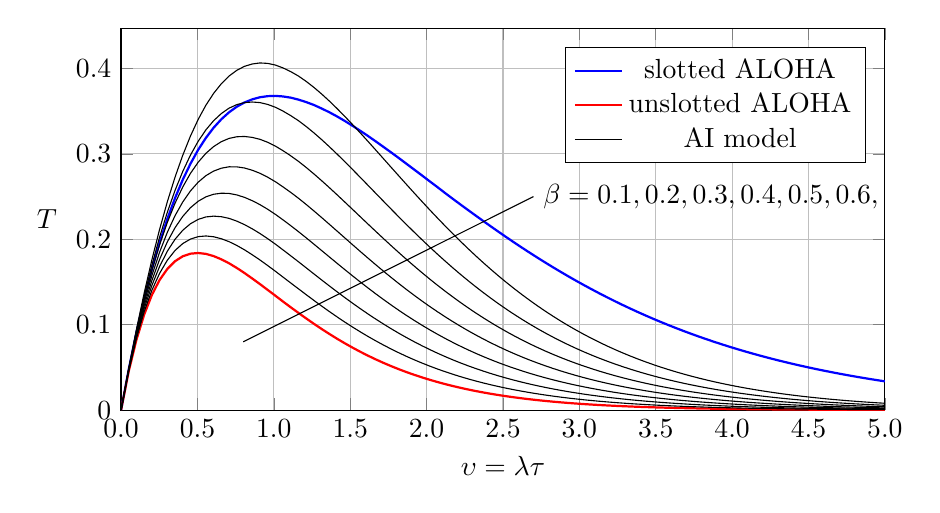
\begin{tikzpicture}[scale=1.0]

\begin{axis}
[
  title={},
  width  = 0.8*\columnwidth, 
  height = 0.4*\columnwidth,
  legend style={at={(0.975,0.95)}, anchor=north east},
%   xmode=log,
  xlabel={$\upsilon=\lambda\tau$},
  ylabel={$\mathscr{T}$}, ylabel style={rotate=-90},
%  yticklabel=\pgfmathprintnumber{\tick}\\ \%,
  xmin = 0, 	
  xmax = 5,
  ymin = 0, 	
%   ymax = 3,
  x tick label style={
        /pgf/number format/.cd,
        fixed,
        fixed zerofill,
        precision=1,
        /tikz/.cd
  },
  grid = both,
  scale only axis,
]
	\legend{slotted ALOHA, unslotted ALOHA, AI model}
    
    \addplot[thick, blue, domain = 0:5, samples=100] {x*exp(-x)};
    \addplot[thick, red, domain = 0:5, samples=100] {x*exp(-2*x)};
    
    \foreach \e in {0.1,0.2,0.3,0.4,0.5,0.6,0.7}
        \addplot[domain = 0:5, samples=100] {x*exp(-2*x)*cosh(sqrt(8*\e*x))/(1+8*\e*x/4)^(1/4)*(1+0.24273*8*\e*x)/(1+0.43023*8*\e*x)};
    
    % \addplot[domain = 0.5:1.04, dashed, samples=100] {x*(1+((-3 + 2*x + sqrt(5 + 4*(-1 + x)*x))/(2*x))*x)*exp(-(2-((-3 + 2*x + sqrt(5 + 4*(-1 + x)*x))/(2*x)))*x)};
    
%     \addplot[thick] table
%     [
% 		x expr = \thisrow{lam},
%     	y expr = \thisrow{25dB}
%     ] {./Data/envelopes.dat};

    \draw[-\arrowhead] (axis cs: 0.8,0.08) -- (axis cs: 2.7,0.25) node[anchor= west] 
        {$\beta = 0.1,0.2,0.3,0.4,0.5,0.6,0.7$};
\end{axis}

\end{tikzpicture}

        \includegraphics[]{Figures/Ch5_AI.pdf}
    \else
        \includegraphics[draft, width=\textwidth]{Figures/placeholder.png}
    \fi
    \caption{Throughput $\mathscr{T}$ of the AI model as a function of occupation rate of the channel $\upsilon$ for different values of $\beta$.}
    \label{fig:P2_AI}
\end{figure}%
%
\begin{figure}[htb]
    \centering
    \if\printfig1
        % \input{Plots/Ch5_AI_ps.tex}
        \includegraphics[]{Figures/Ch5_AI_ps.pdf}
    \else
        \includegraphics[draft, width=\textwidth]{Figures/placeholder.png}
    \fi
    \caption{Parametric curve of the throughput $\mathscr{T}$ and the transmission success probability $p_s$ as we vary $\upsilon$ in the AI model for different values of $\beta$.}
    \label{fig:P2_AI_ps}
\end{figure}

% % % % % % % % % % % % % % % % % % % % % 
\section{High Interference model}
\label{sec:HI_model}

In the High Interference model (HI model) we assume that a packet is successfully transmitted if the proportion of the packet that was affected by \textit{high interference} is smaller than or equal to $\beta\in[0,1]$. We define the period of \textit{high interference} as the times for which the number of interfering packets is greater than a threshold $h\in\N$.

Thus, the transmission success probability is given by $p_s = \P\!\left(\overline{S_h} \le \beta\right)$, where $\overline{S_h}$ is the proportion of time the typical packet was affected by \textit{high interference} and is defined as
\begin{align}\label{eq:Sh_def}
    \overline{S_h} \triangleq \frac{1}{\tau}\int_0^\tau \ind\{I_0(t) > h\}\,\d t.
\end{align}

Considering every $h\in\N$, the distribution of the random variable $\overline{S_h}$ would provide a thorough characterization of the stochastic process $\{I(t)\}_t$,
%
because it would capture every interference level and the distribution of its duration in the typical packet.
%
However, as we shall see, the distribution of $\overline{S_h}$ is quite intricate.

\begin{remark} \label{remark:Ch5_ineq}
    The HI model is a generalization of the ECC model because we recover the latter by making $h=0$ in the former.
    %
    Also, one can show that the HI model is related to the AI model through the following identity
    \begin{align*}
        \sum_{h\ge 0} \overline{S_h} = \overline{I_0}.
    \end{align*}
    Furthermore, $\overline{S_0} \ge \overline{S_1} \ge \cdots$.
\end{remark}

Let the number of interferers that start transmitting during the transmission of the typical packet be represented by the random variable $LI$ (late interferers) and the number of interferers that stop transmitting during the transmission of the typical packet be represented by the random variable $EI$ (early interferers), i.e.,
\begin{align*}
    EI \triangleq I_0(0) \sim \mathscr{P}(\lambda\tau), \qquad LI \triangleq I_0(\tau) \sim \mathscr{P}(\lambda\tau).
\end{align*}
Then, since $\Pi$ is a Poisson point process, it is easy to see that $EI$ and $LI$ are independent and follow a Poisson distribution of parameter $\upsilon = \lambda\tau$.

Let $(t_k)_{k=1}^{EI+LI}$ be the sequence of times for which an interferer stops or starts a transmission.
%
Then, it is possible to uniquely determine $\{I(t)\}_t$ from the sequences $(t_1,\dots,t_{EI+LI})$ and $(I(0),I(t_1),\dots,I(t_{EI+LI}))$.
%
Furthermore, the proportion of time the typical packet was affected by \textit{high interference} can be written as
\begin{align} \label{eq:ch5_Sh}
    \overline{S_h}
        &= \sum_{k=0}^{EI+LI} \dfrac{\Delta t_k}{\tau}\,\ind{\{I(t_k) > h\}},
\end{align}
where $\Delta t_k \triangleq t_{k+1} - t_{k}$ and we use $t_0 = 0$, $t_{EI+LI+1} = \tau$.

Given $EI = k$ and $LI = l$, the distribution of the $k+l$ times of starting or stopping a transmission are independent and uniformly distributed on $[0,\tau)$. 
\begin{note}
    We can check the above-mentioned property by showing the random variable that represents the number of points of the PPP that are in a subset $T$ of $[0,\tau)$ follow a binomial distribution of parameters $(k+l,\mu(T))$, where $\mu(T)$ is the length of the subset.
    
    To prove this property in a more general form, it is enough to show that for every $A,B\in\cal{B}(\R)$ such that $A\subset B$ the random variable $\Pi(A)|\Pi(B)$ follows a binomial distribution of parameters $(\Pi(B), \mu(A)/\mu(B))$ , where $\mu$ is the Lebesgue measure.
\end{note}

Further, the random vector $(I(t_i))_{i=0}^{k+l}$ is a symmetric Bernoulli random walk\footnote{A symmetric Bernoulli random walk is a random walk on $\Z$ that performs unitary steps and each step has equal probability of being $+1$ or $-1$.} subject to begin at $k$ and end at $l$ with $k+l$ steps.
%
% In this random walk, every path is equiprobable.
The total number of different paths is given by the binomial coefficient $\binom{k+l}{k}$.
%
We are interested to know how many of these paths stay a total number of $m\in\N$ steps above the threshold $h$. Let us denote the number of paths that satisfy this as $C_{k,l}^{h,m}\in\N$.
%
Formally, we can write that
\begin{align} \label{eq:Ch5_Cklhm}
    C_{k,l}^{h,m} \triangleq \sum_{\bm{x}\in\mathscr{X}_{k,l}}\ind
        \!\left\{ \sum_{i=0}^{k+l} \ind\{x_i > h\} = m\right\},
\end{align}
where $\mathscr{X}_{k,l} \subset \N^{k+l+1}$ is the set that contains all paths from $k$ to $l$ with $k+l$ unit steps.

Now we can express the probability of having exactly $m$ times of the random vector $(t_i)_{i=0}^{k+l}$ for which the typical packet is affected by an interference greater than $h$ as $C_{k,l}^{h,m}/\binom{k+l}{k}$.

Fig.~\ref{fig:random_walk} illustrate some random walks that starts at $k=5$ and end at $l=3$ in $k+l=8$ steps. We show $3$ of the $\binom{8}{3} = 56$ possible paths.
%
Note that for this case, the only path that surpass $h=7$ (\textit{high interference}) is the red path and it stays above $h$ for only $m=1$ step.
%
Indeed, $C_{5,3}^{7,m} = \ind\{m=1\}$, thus there is only one path that does that.
\begin{figure}[htb]
\centering
    \if\printfig1
        \includegraphics[width=0.45\textwidth]{Figures/Ch5_RandomWalk.pdf}
    \else
        \includegraphics[draft, width=0.5\textwidth]{Figures/Ch5_RandomWalk.pdf}
    \fi
	\caption{Examples of random walks starting at $k=5$ and finishing at $l = 3$.}
	\label{fig:random_walk}
\end{figure}
%
It is worth remembering that in the original problem the $i$th step of the random walk stays in the corresponding state a time given by the random variable $\Delta t_i$.

Different from the other models, the HI model is much more complex, because the calculation of $C_{k,l}^{h,m}$ is done case by case despite having a (strictly speaking) \textit{closed form} expression.
%
As we shall see, we need $C_{k,l}^{r,m}$ for an infinite number of argument combinations and, then, we stumble upon a difficult problem.

\begin{remark} \label{rem:Ch5_Crmkl}
    On the other hand, we can find simple formulas for some special argument values of $C_{k,l}^{r,m}$ as follows.
    \begin{itemize}
        \item $C_{k,l}^{r,m} = C_{l,k}^{r,m}$ by symmetry;
        
        \item If $k\leq r$ and $l\leq r$, then $C_{k,l}^{r,0} = \binom{k+l}{k} - \binom{k+l}{r+1}$ by the reflection method \cite{feller1968introduction};
        
        \item If $k>r$ and $l>r$, then $C_{k,l}^{r,k+l+1} = \binom{k+l}{k} - \binom{k+l}{r}$ by the reflection method again;
        
        \item If $k\leq r$ and $k+l-(r-k) \leq m \leq k+l$, then $C_{k,l}^{r,m}=0$,
    \end{itemize}
    where we consider the binomial coefficient $\binom{n}{k} = 0$ when $k \notin \{0,1,\dots,n\}$.
\end{remark}

Assuming that we have $m$ intervals of time with \textit{high interference}, then we need to find the probability that the sum of $m$ intervals of \textit{high interference} is smaller or equal than $\beta\tau$, which is the condition for successful transmission.
%
Indeed, we have that
\[
    \P(\Delta t_0 + \Delta t_1 + \cdots + \Delta t_{m-1} \leq \beta\tau) = \cal{P}_{k+l,m}(\beta),
\]
where
\begin{align} \label{eq:Ch5_Pdef}
    \cal{P}_{n,m}(x) \triangleq
    \begin{cases}
        \ind\{m = 0\}, &\text{if } x = 0,\\
        \displaystyle\sum_{i=m}^{n} \binom{n}{i}x^i(1-x)^{n-i}, &\text{if } x\in(0,1),\\
        1, &\text{if } x = 1,
    \end{cases}
\end{align}
because we have $k+l$ independent random variables uniformly distributed on $[0,\tau)$ and we want that at least $m$ of them are in the interval $[0,\beta\tau]$.
%
From order statistics theory we can generalize this result to
\begin{align} \label{eq:ch5_Pdeltat}
	\P(\Delta t_{\nu(0)} + \Delta t_{\nu(1)} + \cdots + \Delta t_{\nu(m-1)} \leq \beta\tau) = \cal{P}_{k+l,m}(\beta),
\end{align}
where $\nu:\{0,1,\cdots,m-1\} \longrightarrow \{0,1,\cdots,k+l\}$ is an arbitrary injective function.
%
This takes into account the cases where the intervals of \textit{high interference} are not contiguous.

Finally, we can conclude from \eqref{eq:ch5_Sh} and \eqref{eq:ch5_Pdeltat} that
\begin{align} \label{eq:Ch5_Sh_EIEL}
    \P(\overline{S_h} \leq x~|~EI=k,LI=l) 
	    &= \sum_{m=0}^{k+l+1} \dfrac{C_{k,l}^{r,m}}{\binom{k+l}{k}} \cal{P}_{k+l,m}(x), \quad x\in[0,1].
\end{align}

Now, we are prepared to prove the following theorem.
\begin{theorem} \label{th:F_Sh}
    The cumulative distribution function of $\overline{S_h}$, $h\in\N$, is
    \begin{align*}
        F_{\overline{S_h}}(x)
            &= \euler^{-2\upsilon} \sum_{n \geq 0} \frac{\upsilon^n}{n!} \sum_{m=0}^{n+1}  \cal{P}_{n,m}(x) \sum_{k=0}^n C^{h,m}_{k,n-k}, \quad x\in[0,1],
    \end{align*}
    where $\upsilon = \lambda\tau$, $C$ is defined in \eqref{eq:Ch5_Cklhm} and $\cal{P}$ is defined in \eqref{eq:Ch5_Pdef}.
    
    Further, we can express the probabilities at the discontinuities of $F_{\overline{S_h}}$ in \textit{closed form}:
    \begin{align*}
        \P(\overline{S_h}=0) 
            &= \left( f_{h}(\upsilon) \right)^2 + (\upsilon-h) \frac{\upsilon^{h+1}\euler^{-\upsilon}}{(h+1)!} f_{h}(\upsilon)  - \dfrac{\upsilon^{2(h+1)}\euler^{-2 \upsilon}}{h!(h+1)!},\\
        \P(\overline{S_h}=1) 
            &= \left( 1 - f_{h}(\upsilon) \right)^2 + (h+1-\upsilon) \left( 1 - f_{h-1}(\upsilon) \right) \frac{\upsilon^h \euler^{-\upsilon}}{h!} -(h+1)\frac{\upsilon^{2h}\euler^{-2\upsilon}}{(h!)^2},
    \end{align*}
    where $f_h(\upsilon)\triangleq \euler^{-\upsilon}\displaystyle\sum_{k=0}^{h}\frac{\upsilon^h}{h!}$.
\end{theorem}
\begin{proof}
    We know that the random variables $EI$ and $LI$ follow a Poisson distribution of parameter $\upsilon=\lambda\tau$. Thus, we can decondition \eqref{eq:Ch5_Sh_EIEL} on $EI$ and $LI$ to obtain, for $x\in[0,1]$,
    \begin{align}
    	\P(\overline{S_h} \leq x)
    	    &= \euler^{-2\upsilon}\sum_{k \geq 0}\sum_{l \geq 0} \frac{\upsilon^{k+l}}{k!l!}\sum_{m=0}^{k+l+1} \dfrac{C_{k,l}^{r,m}}{\binom{k+l}{k}} \cal{P}_{k+l,m}(x) \label{eq:Ch5_F_Sh_aux1}\\
    		&= \euler^{-2\upsilon}\sum_{k \geq 0}\sum_{l \geq 0} \frac{\upsilon^{k+l}}{(k+l)!}\sum_{m=0}^{k+l+1} C_{k,l}^{r,m} \cal{P}_{k+l,m}(x) \label{eq:Ch5_F_Sh_aux2}\\
        	&= \euler^{-2\upsilon}\sum_{n \geq 0} \sum_{m=0}^{n+1}  \sum_{k=0}^n C^{r,m}_{k,n-k} \cal{P}_{n,m}(x)  \frac{\upsilon^n}{n!},
    \end{align}
    where we performed the variable change $l=n-k$ and we can interchange the sums because all terms are positive (Fubini–-Tonelli theorem, Theorem~\ref{th:fubini-tonelli}).
    %
    This proves the first result because $F_{\overline{S_h}}(x) = \P(\overline{S_h} \le x).$
    
    Now, using \eqref{eq:Ch5_F_Sh_aux2} and Remark~\ref{rem:Ch5_Crmkl} we have that
    \begin{align*}
    \P(\overline{S_h} = 0)
    	 &= \euler^{-2\upsilon}\sum_{k \geq 0}\sum_{l \geq 0} \frac{\upsilon^{k+l}}{(k+l)!}\sum_{m=0}^{k+l} C_{k,l}^{h,m} \cal{P}_{k+l,m}(0)\\
         &= \euler^{-2\upsilon}\sum_{k \geq 0}\sum_{l \geq 0} \frac{\upsilon^{k+l}}{(k+l)!} C_{k,l}^{h,0}\\
         &= \euler^{-2\upsilon}\sum_{k \geq 0}\sum_{l \geq 0} \frac{\upsilon^{k+l}}{(k+l)!} \left( \binom{k+l}{k} - \binom{k+l}{h+1} \ind_{\{k+l > h\}} \right)\ind_{\{k \leq h\}}\ind_{\{l \leq h\}}\\
         &= \euler^{-2\upsilon}\sum_{k = 0}^h \sum_{l = 0}^h \frac{\upsilon^{k+l}}{k!l!} \left( 1 - \frac{\binom{k+l}{h+1}}{\binom{k+l}{k}} \right).
    \end{align*}
    %
    Now, using $f_h$ and some tedious manipulations we find the \textit{closed form} of $\P(\overline{S_h} = 0)$.
    
    Using \eqref{eq:Ch5_F_Sh_aux1} and Remark~\ref{rem:Ch5_Crmkl} we have that
    \begin{align*}
	\P(\overline{S_h}=1)
	    &= F_{\overline{S_h}}(1) - \lim_{x\uparrow 1} F_{\overline{S_h}}(x)\\
    	&= \euler^{-2\upsilon}\sum_{k > 0}\sum_{l > 0} \frac{\upsilon^{k+l}}{k!l!} \dfrac{C_{k,l}^{h,k+l+1}}{\binom{k+l}{k}}\\
    	&= \euler^{-2\upsilon} \sum_{k > 0}\sum_{l > 0} \frac{\upsilon^{k+l}}{k!l!} \left( 1 - \frac{\binom{k+l}{h}}{\binom{k+l}{k}} \right)\ind_{\{k>h\}}\ind_{\{l>h\}}\\
    	&= \euler^{-2\upsilon} \sum_{k > h}\sum_{l > h} \frac{\upsilon^{k+l}}{k!l!} \left( 1 - \frac{\binom{k+l}{h}}{\binom{k+l}{k}} \right).
    \end{align*}
    %
    Again, using $f_h$ and some tedious manipulations we find the \textit{closed form} of $\P(\overline{S_h} = 1)$.
\end{proof}

Using Theorem~\ref{th:F_Sh} we can find simple expressions for the probability of not receiving \textit{high interference} at all during a typical packet transmission, i.e., $\P(\overline{S_h} = 0)$, for $h=0,1,2,\dots$.
%
\begin{align*}
    \P(\overline{S_0} = 0) &= \euler^{-2\,\upsilon},\\
    \P(\overline{S_1} = 0) &= \left( 1+2\upsilon+{\upsilon}^{2}/2 \right){\euler^{-2\,\upsilon}} ,\\
    \P(\overline{S_2} = 0) &= \left( 1+2\,\upsilon+2\,\upsilon^2+(2/3)\,\upsilon^3+(1/12)\,\upsilon^4 \right){{\euler}^{-2\,\upsilon}},\\
                &~\,\vdots\\
    \P(\overline{S_h} = 0) &= \frac{\upsilon^{2h}\euler^{-2\upsilon}}{h!(h+1)!} + \cal{O}(\upsilon^{2h-1}\euler^{-2\upsilon}), \quad \text{as } \upsilon\to\infty.
\end{align*}

The same can be done for the case of receiving \textit{high interference} during all transmission, i.e., $\P(\overline{S_h} = 1)$.
%
\begin{align*}
    \P(\overline{S_0} = 1) &= 1 - (1+\upsilon)\,\euler^{-\upsilon},\\
    \P(\overline{S_1} = 1) &= (1-\euler^{-\upsilon})^2 - \upsilon^2\,\euler^{-\upsilon},\\
    \P(\overline{S_2} = 1) &= (1-(1+\upsilon)\,\euler^{-\upsilon})^2 + (1-\upsilon-\euler^{-\upsilon})\,\frac{\upsilon^2}{2}\,\euler^{-\upsilon},\\
        &~\,\vdots\\
    \P(\overline{S_h} = 1) &= 1 - \frac{\upsilon^{h+1}}{h!}\,\euler^{-\upsilon} + \cal{O}\left(\upsilon^h\euler^{-\upsilon}\right), \quad \text{as } \upsilon\to\infty.
\end{align*}

\begin{figure}[htb]
    \centering
    \if\printfig1
        \begin{subfigure}{.45\textwidth}
          \centering
            % 
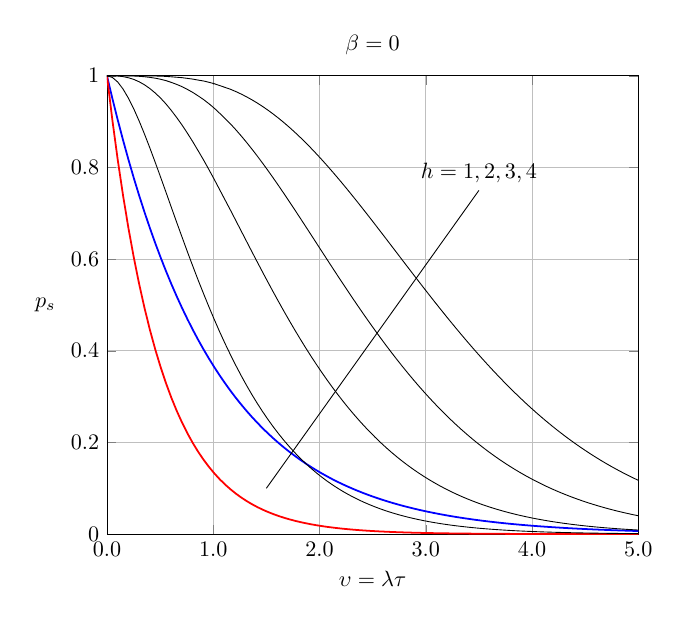
\begin{tikzpicture}[scale=0.8]

\begin{axis}
[
  title={$\beta = 0$},
%   width  = 0.8*\columnwidth, 
%   height = 0.4*\columnwidth,
  legend style={at={(0.95,0.95)}, anchor=north east},
%   xmode=log,
  xlabel={$\upsilon=\lambda\tau$},
  ylabel={$p_s$}, ylabel style={rotate=-90},
%  yticklabel=\pgfmathprintnumber{\tick}\\ \%,
  xmin = 0, 	
  xmax = 5,
  ymin = 0, 	
  ymax = 1,
  x tick label style={
        /pgf/number format/.cd,
        fixed,
        fixed zerofill,
        precision=1,
        /tikz/.cd
  },
  grid = both,
  scale only axis,
]
% 	\legend{slotted ALOHA, unslotted ALOHA}
    
    \addplot[thick, blue, domain = 0:5, samples=100] {exp(-x)};
    \addplot[thick, red, domain = 0:5, samples=100] {exp(-2*x)};
    
    \addplot[domain = 0:5, samples=100] {(1+2*x+x^2/2)*exp(-2*x)};
    \addplot[domain = 0:5, samples=100] {(1+2*x+2*x^2+(2/3)*x^3+x^4/12)*exp(-2*x)};
    \addplot[domain = 0:5, samples=100] {(1+2*x+2*x^2+(4/3)*x^3+(11/24)*x^4+x^5/12+x^6/144)*exp(-2*x)};
    \addplot[domain = 0:5, samples=100] {(1+2*x+2*x^2+(4/3)*x^3+(2/3)*x^4+(13/60)*x^5+(2/45)*x^6+x^7/180+x^8/2880)*exp(-2*x)};
    
%     \addplot[thick] table
%     [
% 		x expr = \thisrow{lam},
%     	y expr = \thisrow{25dB}
%     ] {./Data/envelopes.dat};

    \draw[-\arrowhead] (axis cs: 1.5,0.1) -- (axis cs: 3.50,0.75) node[anchor=south] 
        {$h = 1, 2, 3, 4$};
\end{axis}

\end{tikzpicture}

            \includegraphics[width=\columnwidth]{Figures/Ch5_HI_0.pdf}
            % \caption{$\beta = 0$.}
        \label{fig:HI_0}
        \end{subfigure}%
        \begin{subfigure}{.05\textwidth}
        \hspace{.05\textwidth}
        \end{subfigure}%
        \begin{subfigure}{.45\textwidth}
          \centering
            % 
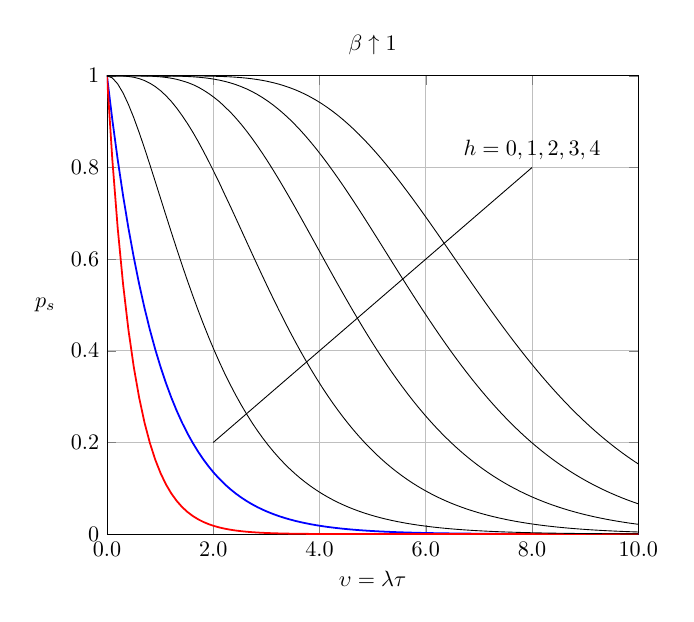
\begin{tikzpicture}[scale=0.8]

\begin{axis}
[
  title={$\beta\uparrow 1$},
%   width  = 0.8*\columnwidth, 
%   height = 0.4*\columnwidth,
  legend style={at={(0.95,0.95)}, anchor=north east},
%   xmode=log,
  xlabel={$\upsilon=\lambda\tau$},
  ylabel={$p_s$}, ylabel style={rotate=-90},
%  yticklabel=\pgfmathprintnumber{\tick}\\ \%,
  xmin = 0, 	
  xmax = 10,
  ymin = 0, 	
  ymax = 1,
  x tick label style={
        /pgf/number format/.cd,
        fixed,
        fixed zerofill,
        precision=1,
        /tikz/.cd
  },
  grid = both,
  scale only axis,
]
% 	\legend{slotted ALOHA, unslotted ALOHA}
    
    \addplot[thick, blue, domain = 0:10, samples=100] {exp(-x)};
    \addplot[thick, red, domain = 0:10, samples=100] {exp(-2*x)};
    
    \addplot[domain = 0:10, samples=100] {(1+x)*exp(-x)};
    \addplot[domain = 0:10, samples=100] {1-((1-exp(-x))^2-x^2*exp(-x))};
    \addplot[domain = 0:10, samples=100] {1-( (1-(1+x)*exp(-x))^2+(1-x-exp(-x))*x^2/2*exp(-x) )};
    \addplot[domain = 0:10, samples=100] {exp(-2*x)/12*(-12-24*x-24*x^2-8*x^3-x^4+2*exp(x)*(12+12*x+6*x^2-2*x^3+x^4))};
    \addplot[domain = 0:10, samples=100] {exp(-2*x)/144*(-144-288*x-288*x^2-192*x^3-66*x^4-12*x^5-x^6+6*exp(x)*( 48+48*x+24*x^2+8*x^3-3*x^4+x^5 ))};
    % \addplot[domain = 0.5:1.04, dashed, samples=100] {x*(1+((-3 + 2*x + sqrt(5 + 4*(-1 + x)*x))/(2*x))*x)*exp(-(2-((-3 + 2*x + sqrt(5 + 4*(-1 + x)*x))/(2*x)))*x)};
    
%     \addplot[thick] table
%     [
% 		x expr = \thisrow{lam},
%     	y expr = \thisrow{25dB}
%     ] {./Data/envelopes.dat};

    \draw[-\arrowhead] (axis cs: 2,0.2) -- (axis cs: 8,0.8) node[anchor=south] 
        {$h =0,1,2,3,4$};
\end{axis}

\end{tikzpicture}

            \includegraphics[width=\columnwidth]{Figures/Ch5_HI_1.pdf}
            % \caption{$\beta \uparrow 1$.}
        \label{fig:HI_1}
        \end{subfigure}
    \else
        \includegraphics[draft, width=\textwidth]{Figures/placeholder.png}
    \fi
    \caption{Transmission success probability $p_s$ as a function of traffic $\upsilon$ in the HI model. The blue and red curves represent the slotted and unslotted ALOHA, respectively.} \label{fig:HI}
\end{figure}

As shown in the plots of Fig.~\ref{fig:HI}, the transmission success probability $p_s$ increases with $h$, because more concurrent interfering transmissions are necessary to cause \textit{high interference} in the typical packet transmission.

When we fix the threshold $h$ and let the traffic $\upsilon\to\infty$, we have that ${\P(\overline{S_h}=0)=0}$ and $\P(\overline{S_h}=1)=1$.
%
On the other hand, when we fix $\upsilon$ and let $h\to\infty$, then ${\P(\overline{S_h}=0)=1}$ and $\P(\overline{S_h}=1)=0$.
%
Thus, an interesting scenario to analyse is what happens when we increase the traffic $\upsilon$ along with the threshold $h$, i.e., let $\upsilon\to\infty$ and $h\to\infty$ such that $\frac{h}{\upsilon} \to 1$.
%
In this case we can show that
\begin{align*}
   \lim_{\substack{h,\upsilon\to\infty\\ h/\upsilon\to1}} \P(\overline{S_h} = 0) &=  \lim_{\substack{h,\upsilon\to\infty\\ h/\upsilon\to1}} \P(\overline{S_h} = 1) = \frac{1}{4}\left( 1 - \frac{2}{\pi}\right) \approx 0.091.
\end{align*}

\begin{note}
    To find the above result it is necessary to calculate an interesting limit problem, which cannot be solved through standard techniques, indeed the Software \textit{Mathematica} (version 12) does not solve it. In a simpler form, the problem is to show that
    \begin{align*}
        \lim_{n\to\infty} f_n(n) = \lim_{n\to\infty} \frac{\Gamma(n,n)}{\Gamma(n)} = \frac{1}{2},
    \end{align*}
    where $\Gamma(\cdot,\cdot)$ is the incomplete gamma function and is defined as $\Gamma(s,x)\triangleq \int_{x}^\infty t^{s-1} \euler^{-t}\,\d t$, and $\Gamma(\cdot) \triangleq \Gamma(\cdot,0)$ is the gamma function.
    
    To prove this identity we use the central limit theorem!
    
    Let $\{X_k\}_k$ be iid exponentially distributed random variables with parameter $1$. Let the sum $S_n = \sum_{k=1}^n X_k$, then $S_n$ follows an Erlang distribution of parameters $(n,1)$. Then, $\P(S_n > n) = \frac{\Gamma(n,n)}{\Gamma(n)}$. However, $\P(S_n > n) = \P(\frac{S_n-n}{\sqrt{n}} > 0) \xrightarrow{n\to\infty} 1/2$ by the central limit theorem.
\end{note}

To conclude this part, let us state the following inequalities, for $\beta > 0$, $\upsilon > 0$, $h\ge 0$,
\begin{align*}
    p_s^{\mathrm{(ALOHA)}} &\le p_s^{\mathrm{(ECC)}} \le p_s^{\mathrm{(AI)}} \le p_s^{\mathrm{(HI)}},\\
    \mathscr{T}^{\mathrm{(ALOHA)}} &\le \mathscr{T}^{\mathrm{(ECC)}} \le \mathscr{T}^{\mathrm{(AI)}} \le \mathscr{T}^{\mathrm{(HI)}},
\end{align*}
which are easily obtained from Remark~\ref{remark:Ch5_ineq} and the definitions of throughput and transmission success probability.

% % % % % % % % % % % % % % 
\section{Summary} \label{sec:summ_P2_01}

In this chapter, we characterized the distribution of the interference in a typical packet, where interferers transmit according to a Poisson process.
%
The characterization was performed through the analysis of some transmission success models (ECC, AI, HI), for which we obtained the throughput and the transmission success probability in closed form.
%
We also compared the obtained distributions with those of the slotted/unslotted ALOHA.
